\documentclass{article}
\usepackage{graphicx}
%permite ecribir acentos directamente
\usepackage[utf8]{inputenc}
% Esto es para que el LÁTEX sepa que el texto está en español, se agrega el ingles para el paquete de gráfico de circuitos:
\usepackage[spanish]{babel}
\usepackage{geometry}
 \geometry{a4paper,total={170mm,257mm},left=15mm,right=15mm,top=20mm,}
\usepackage{hyperref} 
\usepackage{textcomp}
\usepackage{fancyhdr}
\usepackage{siunitx}
\usepackage{amsmath}
\usepackage{multirow}

\usepackage{tikz}
\usetikzlibrary{shapes,arrows}


\pagestyle{fancy}
\fancyhf{}
\lhead{Tecnología Electrónica}
\rhead{Navarro, Verón}
\rfoot{Page \thepage}
 

\begin{document}
\begin{titlepage}
 \centering
	
\includegraphics[scale=0.80]{imagenes/LOGO.jpg} \par
 	\vspace{1cm}
 	{\scshape\LARGE Universidad Tecnológica Nacional \par}
 	{\scshape\large Facultad Regional de Córdoba \par}
 	\vspace{1cm}
	{\bfseries \Large Trabajo Práctico $N^{\circ} 1$\par}
	{\bfseries \Large Cálculo de confiabilidad de sistemas electrónicos \par}
 	\vspace{1.5cm}

	\begin{tabular}{ll}
		Navarro, Facundo 	&	63809 	\\
		Veron, Misael	 	&	62628
	\end{tabular}
	
	\vspace{1cm}
	Curso: 5r2 \\
 	\vfill
	{\bfseries \Large Cátedra: Tecnología Electrónica \par}

	\vspace{1.5cm}
	Docentes: \par
	Ing. Centeno, Carlos \par
	Ing. Gonzalez Dondo, Diego \par

 	\vfill
	{\large \today\par}
\end{titlepage}

%##################################### INDICE  #####################################################

\tableofcontents
\clearpage

%##################################### INDICE  #####################################################

\section{Introducción}
En términos de la teoría de administración de recursos, la estadística tiene un papel fundamental, los modelos probabilísticos aplicados a grandes muestras tienden a "suavizar" las variaciones individuales por lo que el resultado final es lo suficientemente simple y preciso para el análisis de diseño, lo que constituye una importante herramienta para el fabricante para lanzar un producto mas robusto con mejor imagen comercial, minimiza los costos de garantía y reduce considerablemente la necesidad de retirar un producto del mercado para su re diseño, lo que se traduce en una reducción de tiempo y costos.

En caso de artículos utilizados en sistemas críticos es necesario para que el sistema presente el menor número de fallas posibles, llegando al punto que tener una doble falla sea virtualmente imposible.

En el diseño de cualquier circuito electrónico se debería realizar un previo cálculo de confiabilidad, ya que de esta manera se pone en evidencia las debilidades y fortalezas del mismo. En el siguiente informe se realizará el análisis sobre un circuito utilizando las normas de dos handbook militares, el  HDBK-MIL-217 y el HDBK-MIL-338B, teniendo la ventaja que no se requiere tener el dispositivo construido, permitiendo un análisis preventivo.

\section{Circuito a analizar}
Se eligió el shield de relés de Arduino, el cual es controlado por un microcontrolador de la marca PIC, el modelo 16F886, el conjunto del PIC con el shield se utilizará para el control autónomo de la luminaria de una vivienda, el sistema se encuentra fijo, sin ser sometido a ningún tipo de vibración, en un ambiente estable y expuesto a una temperatura de entre $24^{\circ}$C y $30^{\circ}$C, a continuación se presenta el esquemático:
\begin{figure}[h]
 \begin{center}
	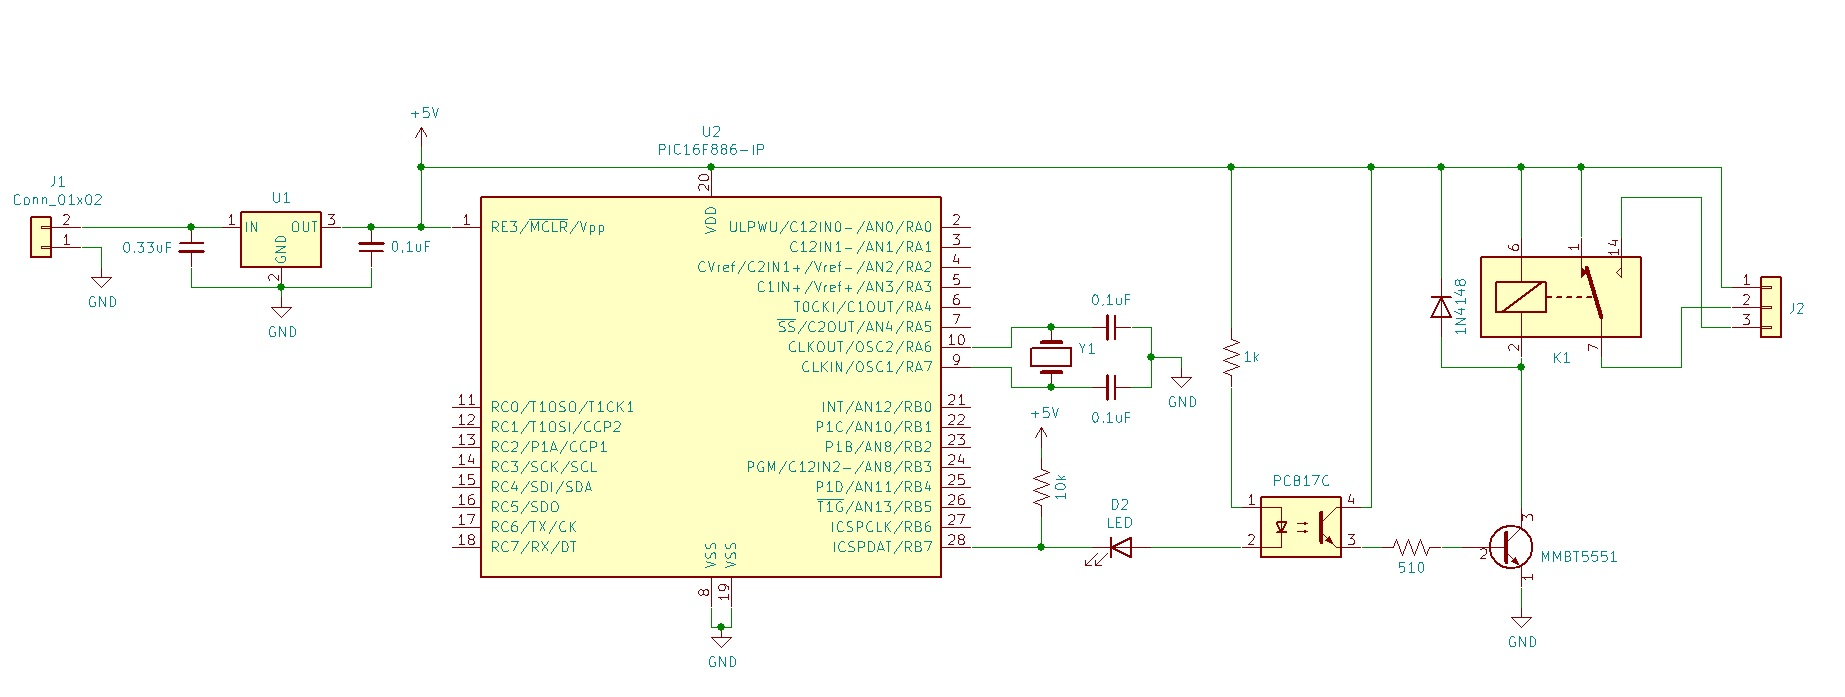
\includegraphics[width=\textwidth]{imagenes/fig1.jpg} 
	\caption{Esquemático del circuito a analizar}\label{fig:fig1}
 \end{center}
\end{figure}
%
\subsection{Lista de Componentes}
Se presenta la lista de componentes que procederemos a analizar secciones mas adelante: \\
\begin{center}
\begin{tabular}{ | c | c | }
  \hline
  Dispostivo & Cantidad \\
  \hline 
    Capacitor 0,1 uF & 3  \\
  \hline 
    Capacitor 0,33 uF & 1  \\
  \hline 
    Regulador de tensión LM7805& 1  \\
  \hline 
    Microcontrolador 16F886 & 1  \\
  \hline
    Cristal  & 1  \\
  \hline
    Resistencias SMD & 3  \\
  \hline
    Diodo LED  & 1  \\
  \hline
    Diodo 1N4148 & 1  \\
  \hline
    Optoacoplador PC817C  & 1  \\
  \hline
    Relé electromecánico  & 1  \\
  \hline
\end{tabular}
\end{center}

\section{Norma MIL-HDBK-217F}
El propósito de este manual es establecer y mantener métodos consistentes y uniformes para estimar la confiabilidad inherente de equipos y sistemas electrónicos militares. Bajo esta norma se establece el tiempo medio entre fallas (MTBF) de dos maneras diferentes, primero se hace el cálculo con respecto al \textit{análisis por stress} el cual tiene en cuenta numerosos parámetros que afectan la vida útil de los componetes, dando como resultado una aproximación mas acertada a la vida útil global, y luego se emplea el método de \textit{cuenta partes} el cual necesita menos información pero tiene la ventaja que es mas generalizado y de mas rápida elaboración.

\subsection{Análisis por Stress}
El método de análisis por stres de la pieza se usa la mayoría del tiempo y es aplicable cuando el diseño está casi terminado y hay una lista detallada de piezas, o BOM, además de la disponibilidad del stress de los componentes. Por stress de componentes, la norma se refiere a las condiciones de operación reales, como el ambiente, la temperatura, la tensión, la corriente y los niveles de potencia aplicados, por ejemplo. El estándar MIL-217 agrupa componentes o partes por categorías principales y luego tiene subgrupos dentro de las categorías. Cada componente o categoría de pieza y sus subgrupos tienen una fórmula o modelo único aplicado para calcular la tasa de falla de ese componente o pieza.

Se desarrollaran cada uno de los componentes, teniendo en cuenta a qué grupo pertenece y su respectiva fórmula para obtener la probabilidad de falla $\lambda_P$ cuya unidad es fallas con respecto a un millón de horas. Con este calculado se procede a calcular el tiempo medio entre fallas o tiempo medio de vida (MTFB) de acuerdo a la siguiente ecuación \ref{eq:lambda}, la cual aplica tanto para elementos individuales o sistemas.

\begin{equation}
MTFB \; = \frac{1}{\lambda_P} \; [Hs] \label{eq:lambda}
\end{equation}

\subsubsection{Diodo 1N4148}
Se calcula de la siguiente manera:

\[\lambda_P = \lambda_b  \cdot \pi_T  \cdot \pi_Q  \cdot \pi_C  \cdot  \pi_S \] 

\begin{center}
\begin{tabular}{ | c | c | c | c | c | c | c | }
  \hline
  Modelo & $\lambda_b$ & $\pi_T$ & $\pi_Q$ & $\pi_C$ &  $\pi_S$ & $\lambda_P$ \\
  \hline
    1N4148 & 0,013 & 32 & 8,0 & 1 &  0,054 & \num{2,2464e-3} \\
  \hline
 \end{tabular}
\end{center}
 
\subsubsection{Transistor Bipolar MMBT5551}
Se calcula de la siguiente manera:

\[\lambda_P = \lambda_b  \cdot \pi_T  \cdot \pi_A  \cdot \pi_R  \cdot \pi_S  \cdot  \pi_Q  \cdot  \pi_E \] 

\begin{center}
\begin{tabular}{ | c | c | c | c | c | c | c | c |  c | }
  \hline
  Modelo & $\lambda_b$ & $\pi_T$ & $\pi_A$ & $\pi_R$ & $\pi_S$ &  $\pi_Q$ &  $\pi_E$  & $\lambda_P$ \\
  \hline
    MMBT5551 & 0,00074 & 8,1 & 0,70 & 0,43 &  0,00142 & 1,0 & 5,5 &  \num{1,409e-5} \\
  \hline
\end{tabular}
\end{center}

\subsubsection{Optoacoplador Pc817c }
Se calcula de la siguiente manera:

\[\lambda_P = \lambda_b  \cdot \pi_T  \cdot \pi_Q  \cdot \pi_E \] 
\begin{center}
\begin{tabular}{ | c | c | c | c | c | c |}
  \hline
  Modelo & $\lambda_b$ & $\pi_T$ & $\pi_Q$ & $\pi_E$ & $\lambda_P$ \\
  \hline
    PC817C & 0,013 & 6,3 & 5,5 & 1,0 &  0,45 \\
  \hline
\end{tabular}
\end{center}

\subsubsection{Relé Electromecánico SRD-05VDC-SL}
Se calcula de la siguiente manera:

\[\lambda_P = \lambda_b  \cdot \pi_L  \cdot \pi_C  \cdot \pi_{CYC}  \cdot \pi_F  \cdot \pi_Q  \cdot \pi_E \] 

\begin{center}
\begin{tabular}{ | c | c | c | c | c | c | c | c | c |}
  \hline
  Modelo & $\lambda_b$ & $\pi_L$ & $\pi_C$ & $\pi_{CYC}$ & $\pi_F$ & $\pi_Q$ & $\pi_E$ & $\lambda_P$ \\
  \hline
    SRD-05VDC-SL & 0,0061 & 0,7 & 1,75 & 1,0 & 1,5 & 8 & 2,0 & 0,17 \\
  \hline
\end{tabular}
\end{center}

\subsubsection{LED SMD VLMW11R2S2}
Se calcula de la siguiente manera:

\[\lambda_P = \lambda_b  \cdot \pi_T  \cdot \pi_Q  \cdot \pi_E \] 
\begin{center}
\begin{tabular}{ | c | c | c | c | c | c |}
  \hline
  Modelo & $\lambda_b$ & $\pi_T$ & $\pi_Q$ & $\pi_E$ & $\lambda_P$ \\
  \hline
    VLMW11R2S2 & 0,00023 & 5,3 & 5,5 & 1,0 & \num{6,7045e-3} \\
  \hline
\end{tabular}
\end{center}

\subsubsection{Resistores}
Se calcula de la siguiente manera:

\begin{center}
\begin{tabular}{ | c | c | c | c | c | c |}
  \hline
  Modelo & $\lambda_b$ & $\pi_{R}$ & $\pi_Q$ & $\pi_E$ & $\lambda_P$ \\
  \hline
    1 k$\Omega$ & 0,00022 & 1,0 & 15 & 1,0 & \num{3,3e-3} \\
  \hline
    10 k$\Omega$ & 0,00022 & 1,0 & 15 & 1,0 & \num{3,3e-3} \\
  \hline
    510 $\Omega$ & 0,00031 & 1,0 & 15 & 1,0 & \num{4,65e-3} \\
  \hline
\end{tabular}
\end{center}

\subsubsection{Capacitores}
Se calcula de la siguiente manera:

\[ \lambda_P = \lambda_b  \cdot \pi_{Cv}  \cdot \pi_Q  \cdot \pi_E \] 

\begin{center}
\begin{tabular}{ | c | c | c | c | c | c |}
  \hline
  Modelo & $\lambda_b$ & $\pi_{Cv}$ & $\pi_Q$ & $\pi_E$ & $\lambda_P$ \\
  \hline
    0,33 uF & 0,00097 & 0,29 & 7,0 & 1,0 & \num{1,96e-3} \\
  \hline
    0,1  uF & 0,00097 & 0,259 & 7,0 & 1,0 & \num{1,75e-3} \\
  \hline
\end{tabular}
\end{center}

\subsubsection{Microcontrolador 16F886}
Se calcula de la siguiente manera:

\[\lambda_P = (C_1  \cdot \pi_T + C_2  \cdot \pi_E)  \cdot \pi_Q \cdot \pi_L \] 

\begin{center}
\begin{tabular}{ | c | c | c | c | c | c | c | c |}
  \hline
  Modelo & $C_1$ & $\pi_T$ & $C_2$ & $\pi_E$ & $\pi_Q$ & $\pi_L$ & $\lambda_P$ \\
  \hline
    16F886 & 0,14 & 5,5 & 0,0014 & 0,5 & 1 & 1,0 & 0,7707 \\
  \hline
\end{tabular}
\end{center}

\subsubsection{Cristal de Quarzo}
Se calcula de la siguiente manera:

\[\lambda_P = \lambda_b  \cdot \pi_Q  \cdot \pi_E \] 
\begin{center}
\begin{tabular}{ | c | c | c | c | c |}
  \hline
  Modelo & $\lambda_b$ & $\pi_Q$ & $\pi_E$ & $\lambda_P$ \\
  \hline
    8Mhz & 0,022 & 2,1 & 1,0 & 0,0462 \\
  \hline
\end{tabular}
\end{center}

\subsubsection{Regulador de Tensión LM7805}
Se calcula de la siguiente manera:

\[\lambda_P = (C_1  \cdot \pi_T + C_2  \cdot \pi_E)  \cdot \pi_Q  \cdot \pi_L \] 

\begin{center}
\begin{tabular}{ | c | c | c | c | c | c | c | c |}
  \hline
  Modelo & $C_1$ & $\pi_T$ & $C_2$ & $\pi_E$ & $\pi_Q$ & $\pi_L$ & $\lambda_P$ \\
  \hline
    LM7805 & 0,010 & 180 & 0,00027 & 0,5 & 0,25 & 1,0 & 0,0453375 \\
  \hline
\end{tabular}
\end{center}

\subsubsection{$\lambda_{pT}$ del sistema}
A partir de cada $\lambda_P$ se puede obtener el  $\lambda_{pT}$ del sistema mediante la sumatoria de cada uno de ellos multiplicado por un factor $n$ correspondiente a la cantidad de veces que se repite, de modo que:

\begin{align*}
\lambda_{pT} =&\lambda_{C0,33uF} + 3 \cdot \lambda_{C0,1uF} + \lambda_{LM7805} \; + \lambda_{Crystal} \;+\; \lambda_{16F886} \;+\; \lambda_{R10k} \;+\;\\
			  &\lambda_{R1k} \;+\; \lambda_{R510} \;+\; \lambda_{1N4148} \;+\; \lambda_{rele} \;+\; \lambda_{BJT} \;+\; \lambda_{optoacoplador} \;+\; \lambda_{LED} \\
\lambda_{pT} =&1,85437049 
\end{align*}

Quedando finalmente como vida media:

\begin{align*}
{MTBF}\bigr|_{Sistema} 	&= \frac{\num{e6}}{\lambda_{pT}} \\
						&= \frac{\num{e6}}{1,85437049 } \\
						&= 39266,5626  \; [Hs] \\
						&= 22469,44  \;   [Dias] \\
{MTBF}\bigr|_{Sistema}	&= 615,60 \;  [A\tilde{n}os] 
\end{align*}

Esto indica que nuestro circuito tiene una vida media de aproximadamente 62 años, puede durar más o menos, pero nos da la certeza que  la probabilidad de falla de la mayoría de nuestros circuitos oscilará en un período de 62 años.

\subsection{Análisis por cuenta partes}
El método de análisis de cuentas partes requiere menos información,tal como cantidades de piezas, nivel de calidad y entorno de aplicación. Es más aplicable durante las fases iniciales de diseño o propuesta de un proyecto. 

El estándar MIL-217 proporciona tablas para los grupos de componentes (los mismos grupos que el análisis por stress) que enumeran las tasas de falla y los factores de calidad genéricos para los diferentes entornos MIL-217.

El análisis de recuento de piezas no tiene en cuenta las numerosas variables y utiliza las tasas de falla genéricas o de base más desfavorables y los factores $\pi$. El Método de cuenta de partes generalmente resultará en una mayor tasa de fallas o en una menor confiabilidad del sistema, lo que brinda un resultado más conservador que el que generaría el método de stress.

Para este cálculo se utiliza la siguiente ecuación:
\begin{equation}
	\lambda_{Pequip} = \sum_{1}^{n} i N_i  \cdot (\lambda_g  \cdot \pi Q) i
\end{equation}

\begin{center}
\begin{tabular}{| c | c | c | c | c | c |}
\hline
Componentes & $N_i$ & $\lambda_g$ & $\pi Q$ & $\lambda_p$ & MTBF [Hs] \\
\hline
LM7805 & 1 & 0,0036 & 0,25 & \num{9e-4} & 2205979,625 \\
\hline
Capacitor cerámico & 4 & 0,0036 & 10 & 0,144 & 69444444,44 \\
\hline
Cristal Quarzo & 1 & 0,0032 & 2,1 & \num{6,32e-3} & 1488095238 \\
\hline
Microcontrolador & 1 & 0,048 & 0,25 & 0,012 & 833333333,3 \\
\hline
Resistencia carbon & 3 & 0,0019 & 10 & 0,057 & 175438596,5 \\
\hline
LED & 1 & 0,00047 & 5,5 & \num{2,5855e-3} & 3868471954 \\
\hline
Optoacoplador & 1 & 0,027 & 5,5 & 0,1485 & 67340067,34 \\
\hline
BJT & 1 & 0,00015 & 5,5 & \num{8,25e-4} & \num{1,21e10} \\
\hline
Rele & 1 & 0,13 & 9,0 & 1,17 & 8547008,547 \\
\hline
Diodo 1N4148 & 1 & 0,0029 & 5,5 & 0,01595 & 626959247,6 \\
\hline
\multicolumn{4}{|c|}{$\lambda_{Pequi}$} & 1,5580805 & 6418453,619\\
\hline
\end{tabular}
\end{center}

como previamente se hizo con la ecuación \ref{eq:lambda},
\begin{align*}
{MTBF}\bigr|_{Sistema} 	&= \frac{\num{e6}}{\lambda_{Pequi}} \\
						&= \frac{\num{e6}}{1,5580805 } \\
						&= 6418453,619  \; [Hs] \\
						&= 267423,06  \;   [Dias] \\
{MTBF}\bigr|_{Sistema}	&= 732,66 \;  [A\tilde{n}os] 
\end{align*}
Aquí se pone en evidencia lo antes expuesto, la vida media difiere ya que los métodos consideran distinta variables, siendo el análisis por stress el más fidedigno, ya que considera mayor cantidad de aspectos reales, aunque para ser un sistema tentativo el método por cuenta partes cumple su función, en nuestro caso expone la longevidad del correcto funcionamiento de nuestro circuito.

\subsubsection{Análisis del modo de fallas y sus efectos FMEA}
El análisis de modos de fallas y efectos (Failure Mode and Effect Analysis) es un método utilizado para prevenir fallas y analizar los riesgos de un proceso mediante la identificación de causas y efectos a fin de determinar las acciones que se utilizaran para inhibir las fallas

El modo de fallas está relacionado con el hecho de como un proceso puede ser llevado a operar de manera deficiente y está compuesto por tres elementos:
 
\begin{itemize}\itemsep0em \itemindent=2em
  \item Efecto
  \item Causa
  \item Detección  
\end{itemize}

El efecto es la consecuencia de lo que la falla puede causar, la causa es lo que indica la razón por la que se produjo el error y la detección es la forma utilizada en el control del proceso para evitar las posibles fallas.

\begin{center}
\begin{tabular}{| c | c | c | c | c |}

\hline
Componente & $\alpha$ & Modo de falla & $\beta$ \\ 
\hline
\multirow{3}*{Diodo 1N4148} 	& 0,51 &		Abierto 					& No elimina transitorios 		& 0,1 					\\
								\cline{2-4}
								& \multirow{2}*{Corto}		& No enciende relé				& \multirow{2}*{1} 		\\
	
								&							& Aumenta $I_C$ de transistor	& 						\\
\hline
\multirow{3}*{Capacitores C1 y C2}				& Abierto					& \multirow{3}*{7805 no estable}				& \multirow{3}*{0,1}	\\
												\cline{2-2}
												& Corto				 		&											&						\\
												\cline{2-2}
												& Cambio de valor			&											&						\\
\hline
\multirow{3}*{Capacitores C3 y C4}				& Abierto					& \multirow{3}*{Oscilador no estable}				& \multirow{3}*{1}	\\
												\cline{2-2}
												& Corto				 		&											&						\\
												\cline{2-2}
												& Cambio de valor			&											&						\\
\hline




\end{tabular}
\end{center}



\end{document}

